\documentclass[10pt,a4paper]{article}
\usepackage[utf8]{inputenc}
\usepackage{amsmath}
\usepackage{amsfonts}
\usepackage{amssymb}
\usepackage{amsthm}



\usepackage{float}
\usepackage{subfigure}
\usepackage{framed}
\usepackage{xcolor}

\usepackage{hyperref}
\hypersetup{
  colorlinks   = true, %Colours links instead of ugly boxes
  urlcolor     = red, %Colour for external hyperlinks
  linkcolor    = black, %Colour of internal links
  citecolor   = blue %Colour of citations
}

\usepackage{graphicx}
\graphicspath{{images2/}}

\definecolor{shadecolor}{gray}{0.9}

% Operators
\DeclareMathOperator*{\argmax}{arg\,max}
\DeclareMathOperator*{\argmin}{arg\,min}
\DeclareMathOperator*{\argminA}{arg\,min} % Jan Hlavacek

% Environments theorems
\newtheorem{questions}{Question}
\newenvironment{question}
   {\begin{shaded}\begin{questions}}
   {\end{questions}\end{shaded}}

\author{Ram\'on Mart\'inez}
\title{BCPNN and Sequence Learning}

% Paragraph parameters
\setlength{\parskip}{1em}

\begin{document}
\maketitle

\section{Introduction}
Actions performedi n the world are at a fundamental level embedded in time. In that light, it is not surprising that neuroscience that neuroscience has a long standing history of interesiting on the representation of time in the brain (cite buonomano) and the relationship between the structure of thought and time (dehane, and Lashely). Why sequence learning in particular. 

Generalities about the necessity of including sequence processing capabilities on our models. Language, movement, music, Lashley.

Stereotyped sequences of activities have been observed. 

Describe attrctors models for sequences. Early on Hopfield noted that assymetry in an attractor neural network will lead to sequential activity \cite{hopfield1982neural} \cite{hopfield1984neurons} \cite{amari1972learning}  \cite{kleinfeld1986sequential} \cite{sompolinsky1986temporal} \cite{amit1992modeling} and their shortcomings.

Sequence modelling in computational neuroscience \cite{veliz2015networks}, \cite{fiete2010spike},
 \cite{murray2017learning} \cite{verduzco2012model}, \cite{wang2017model} \cite{pereira2018unsupervised}

Describe the other attempts at our lab, maybe?

About the relevant temporal scales, Uppi \cite{bhalla2017dendrites}, \cite{paton2018neural}. Systematic justifcation for being interested on sequences at the level we are interested. 

Describe what exactly you are going to do: introduce the model, explain the architecture, show that it possess wide dynamical range, then show that it can learn sequences and characterize this process, describe its how sensitivity it is to noise, show that it can learn non-orthogonal representation. 


\section{Results}
\subsection{Sequence recall}

Following previous work in cortical modelling \cite{tully2016spike, lundqvist2006attractor} we present here a cortical-like network capable of learning, recalling and processing sequential activity. We utilize a population model of the cortex where units represent aggregations of neurons (cortical columns). Consistently with the mesoscale neuroanatomical organization, those units are organized into hypercolumns, where winner-takes-all (WTA) dynamics keeps the activity within the module normalized \cite{douglas2004neuronal}. The topological organization of the model is presented in Fig. \ref{fig:networks_scheme}A. The circuit implements attractor dynamics \cite{lansner2009associative} that leads the evolution of the network towards temporary or permanent patterns of activity. We refer to these stable or meta-stable states as the stored patterns of the network. The patterns themselves are defined by self-recurrent excitatory connectivity that tend to maintain the pattern in place once activated (represented by $w_{self}$ in Fig. \ref{fig:networks_scheme}B). The patterns can naturally be thought of as cell assemblies distributed among the hypercolumns in the network. The WTA mechanism renders the activity of the units mutually exclusively within the hypercolumns and therefore ensures sparse activity \cite{foldiak2003sparse}. Sequential activation of patterns can be induced by feed-forward excitation (represented by $w_{next}$ in Fig. \ref{fig:networks_scheme}B) coupled with an adaptation mechanism whose role is to cease current pattern activity thereby counteracting the pattern retention effects of the self-recurrent connectivity. 

\begin{figure}[H]
\centering
\includegraphics[scale=1.0]{paper_diagram.pdf}
\caption{Network architecture and connectivity underlying sequential pattern activation. (A) network topology. Units $u_i^j$ are organized into hypercolumns $H_1$, $\ldots$, $H_n$. At each point in time only one unit per hypercolumn is active due to a WTA mechanism. Each memory pattern is formed by a set of recurrently connected units distributed across hypercolumns. For simplicity and without compromising the generality we adopt the convention $P_1=(u_1^1, \ldots, u_1{^n})$. We depict stereotypical network connectivity by showing all the units that emanate from unit $u_1^{1}$. The unit has excitatory projections to the proximate units on the sequence (connections from $u_1^{(1)}$ to $u_2^{(1)}$ and $u_3^{(1)}$ and the corresponding units in other hypercolumns) and inhibitory projections to both the units that are farther ahead on the sequence ($u_1^{(1)}$ to $u_4^{(1)}$) and the units that are not in the sequence at all (gray units). (B) abstract representation of the relevant connectivity for  sequence dynamics. Please not that only connections from $P_2$ are shown.}
\label{fig:networks_scheme}
\end{figure}

We model the dynamics of the units with a population model equation \cite{wilson1972excitatory}. As described in Eq. \ref{eq:current} the current $s$ changes according to the base rate $\beta_i$ plus the total incoming current from the other units $ \sum_{j} w_{ij} o_j$. The binary activation variable $o_i$ represents unit activation and is related to the current through the WTA dynamics described in Eq. \ref{eq:non-linearity}. This  mechanism selects the unit receiving the maximum current at each hypercolumn and activates it. We introduce intrinsic adaptation as a mechanism controlled by the variable a in Eq. \ref{eq:adaptation} to induce pattern deactivation. $d\xi$ represents additive white noise with variance $\sigma$. An extra current $I_i(t)$ is used to model external input into the system. For the sake of generality, it is important to stress that our current based population model is equivalent to a rate-based formalism as shown in \cite{miller2012mathematical}. 


\begin{align}
\tau_s \dfrac{ds_i}{dt} &= \beta_i + \sum_{j} w_{ij} o_j  - g_a a_i - s_i  + \sigma d\xi(t) + I_i(t) \label{eq:current} \\ o_i &=   \begin{cases}
       1,&  s_i = \underset{hypercolumn}{\max}(\mathbf{s}),\\
       0 ,& \text{otherwise}
    \end{cases} \label{eq:non-linearity} \\
\tau_a \dfrac{da_i}{dt} &= o_i - a_i \label{eq:adaptation} 
\end{align}


It has long been recognized that an attractor model with assymetric connectivity produces sequential dynamics \cite{amit1992modeling}. In that vein, we explain now how an asymmetric connectivity matrix coupled with the dynamics of our model brings about sequential activity. 
 
In Fig. \ref{fig:recall}A we show a case of successful sequential recall in the network with the connectivity matrix depicted in  Fig. \ref{fig:recall}D. Here we handcrafted the connectivity matrix to illustrate the unfolding of the following dynamics. Once the first pattern gets activated ($o_i$=1) as a result of an external cue (current input $I(t)$ to all the units belonging to the pattern) the adaptation current $a_i$ depicted in Fig. \ref{fig:recall}B starts growing and, in consequence, self-excitatory current $s_i$ becomes smaller. At some point, the self-excitatory current $s_i$ is going to become weaker than the feed-forward current $s_{i + 1}$ which the next pattern in the sequence is receiving. Then, the competitive WTA mechanism mediates the activation of the next pattern ($o_{i + 1} = 1$) and suppresses the current one ($o_{i}$) by normalization. These dynamics are self-sustained and the cycle repeats until the end of the sequence. We depict the profile of such transitions in Fig.\ref{fig:recall}C. The total time that the pattern stays activated is defined as the persistent time $T_{per}$ (also called dwelling time) and depends on the interplay between the connectivity matrix, the bias term and the adaptation.


\begin{figure}[H]
\centering
\includegraphics[scale=0.25]{simple_bcpnn_recall.pdf}
\caption{An instance of sequence recall in the model. (A) Sequential activity of units initiated by the cue. (B) The time course of the adaptation current for each unit. (C) The total current $s$ (note that this quantity crossing the value of $w_{next} o$ depicted here with a dotted line) marks the transition point from one pattern to the next. (D) The connectivity matrix where we have included pointers to the most important quantities $w_{self}$ for the self-excitatory weight, $w_{next}$ for the inhibitory connection to the next element, $w_{rest}$ for the largest connection in the column after $w_{next}$ and $w_{back}$ for the connection to the last pattern that was active in the sequence.}
\label{fig:recall}
\end{figure}

\subsection{Persistent time}

Two important characteristics of sequence dynamics are the order in which the patterns are activated (the serial order) and the temporal structure of those activations (the temporal order) \cite{dominey2000neural}. 
In our model the serial order is determined by the differential connectivity between the current activated pattern and all other patterns. In general, the next pattern activated will be the one for which the quantity $\Delta w_{next}  = w_{self} - w_{next}$ is smaller. The persistent time or temporal information of the sequence on the other hand is determined by the interplay between the connectivity of the network and the dynamical parameters of the network. We now proceed to characterize  this relationship analytically. From the deterministic trajectories (Eq. \ref{eq:deterministic_solution} in the Appendix) we can find the time point at which the currents from two subsequent units are equal: $s_i(t) = s_{i + 1}(t)$. Solving for $\textit{t}$ we determine the persistent time, $T_{per}$ for each attractor determined with the expression in Eq. \ref{eq:persistent_times}.  

\begin{align}
T_{per} &= \tau_a \log \left(\frac{1}{1 - B} \right) + \tau_a \log \left( \frac{                                                                                                                                                                                     1}{1 - \frac{\tau_s}{\tau_a}} \right) \label{eq:persistent_times}  \\ 
B &= \frac{w_{self} - w_{next} + \beta_{self} - \beta_{next}}{g_a} \label{eq:B_parameter} \\  
 &= \frac{\Delta w_{next} + \Delta \beta_{next}}{g_a} \nonumber  
\end{align}


The parameter B in Eq. \ref{eq:B_parameter} condenses information regarding the connectivity $w$, bias terms $\beta$, and adaptation strength $g_a$. From Eq. \ref{eq:persistent_times} we can infer that $T_{per}$ is defined only for $0 < B < 1$. This sets the conditions for how the weights, bias and external input interact with the adaptation parameters in order for the sequence to be learned and recalled. The straightforward interpretation for $B < 1$ is that the adaptation has to be strong enough to overcome the effects of the other currents. We summarize the effect of B on the $T_{per}$ in Fig. \ref{fig:per_time}. As illustrated in Fig. \ref{fig:per_time}A $T_{per}$ is small for $B \approx 0$ and diverges to infinity as $B \approx 1$. This facilitates the interpretation of $B$ as a unitless parameter whose natural interpretation is the inverse of transition speed, as shown in the examples provided in Fig. \ref{fig:per_time}B-C.

Controlling the individual persistent times of different patterns (the temporal structure) through short-term dynamics has been discussed previously in the literature \cite{veliz2015networks}. In our model the temporal structure of the sequence is also controlled  by the adaptation dynamics. Choosing specific values of $g_a$ for different units allow us to control $T_{per}$ for every atractor in a precise way, as illustrate in Fig. \ref{fig:per_time}D. 


\begin{figure}[H]
\centering
\includegraphics[scale=0.30]{persistent_times.pdf}
\caption{Systematic study of persistent time $T_{per}$. (A) $T_{per}$ dependence of B. The blue solid line represents the theoretical prediction described in Eq. \ref{eq:persistent_times} and the orange bullets are the result of simulations. (B) An example of sequence recall where $T_{per}=100 \: ms$. This example corresponds to configuration marked the black star in (A). (C) example of sequence recall with $T_{per}=500 \: ms$. This example corresponds to the configuration marked with a black triangle in (A). (D) Recall of a sequence with variable temporal structure (varying $T_{per}$. The values of $T_{per}$ are $500$, $200$, $1200$, $100$, and $400 $ ms respectively.}
\label{fig:per_time}
\end{figure}

\subsection{Learning}

So far we have shown that our model can support sequence recall and control of the temporal structure through the adaptation dynamics. We now show that if the network is subject to the right spatio-temporal input structure then associative Hebbian learning is sufficient to induce the learning of the asymmetric connectivity structure characteristic of sequence recall \cite{amit1992modeling}. Based on previous work \cite{tully2016spike} we use the the BCPNN learning rule  in its incremental on-line version \cite{sandberg2002bayesian} with learning mediated through asymmetric synaptic time traces. The version of the BCPNN learning rule presented is an adaptation of the discrete learning rule presented in \cite{lansner1989one} to a continuous setting. 

\begin{align}
\tau_{z_{pre}} \dfrac{dz_i}{dt} &= o_i - z_i 
& \tau_{z_{post}} \dfrac{d z_j}{dt} &= o_j - z_j \label{eq:z_traces} \\
t \dfrac{dp_i}{dt} &= z_i - p_i  
\qquad \quad t\dfrac{dp_{ij}}{dt} = z_i z_j - p_{ij}
&t\dfrac{dp_j}{dt} &= z_j - p_j    \label{eq:p_traces} \\
w_{ij} &= \log \left(\frac{p_{ij}}{p_i p_j} \right) & \beta_i &= \log(p_i) \label{eq:bcpnn} 
\end{align}

In the spirit of associative learning the BCPNN rule sets positive weights of recurrent connections between units that statistically tend to co-activate and creates inhibitory connections (negative weights) between those that do not. This is reflected in Eq. \ref{eq:bcpnn}, where the connections are determined with a logarithmic ratio between the probability of co-activation ($p_{ij}$) and the product of the activation probabilities ($p_i$ and $p_j$). Note that if the events are independent the weight between them is zero ($p_{ij}=p_i p_j)$. Nevertheless, basic associative learning can only bind units that are active simultaneously. In order to bind units that are not simulanously active we need an extra mechanism of temporal integration \cite{amit1992modeling}. To overcome this we combine the BCPNN learning rule with the introduction of the z-traces in order to create temporal associations between units that are contigious in time \cite{tully2016spike}. The z-traces, defined in Eq. \ref{eq:z_traces}, which can be thought of as synaptic traces, are a low-passed filtered version of the activation units $o$ and dynamically track the activation as shown in the top of Fig. \ref{fig:learning}B. To approximate the probabilities of activation ($p_i$ and $p_j$) and co-activation ($p_{ij}$) the z-traces are averaged over time in agreement with Eq. \ref{eq:p_traces} which implements an on-line version of the average function. As illustrated in Fig. \ref{fig:learning}A, asymmetry in the connectivity matrix arises from having two z-traces, a pre-synaptic trace with a slow time constant $\tau_{z_{pre}}$ and a fast post-synaptic trace with a fast time constant $\tau_{z_{post}}$. In short, the z-traces work as a temporal proxy for unit activation that allow us to use the probabilistic framework of the BCPNN rule to learn the sequential structure of the input.


%\begin{align}
%\tau_{z_{post}} \dfrac{d\underset{post}{z_i}}{dt} &= o_i - \underset{post}{z_i} 
%& \tau_{z_{pre}} \dfrac{d\underset{pre}{z_i}}{dt} &= o_i - \underset{pre}{z_i} \label{eq:z_traces} \\
%t \dfrac{dp_i}{dt} &= \underset{pre}{z_i} - p_i  
%\qquad \quad t\dfrac{dp_{ij}}{dt} = z_i z_j - p_{ij}
%&t\dfrac{dp_i}{dt} &= \underset{pre}{z_i} - p_i    \label{eq:p_traces} \\
%w_{ij} &= \log(\frac{p_{ij}}{\underset{pre}{p_i} \quad\underset{post}{ p_j}}) & \beta_i &= \log(p_i) \label{eq:bcpnn} 
%\end{align}
 

\begin{figure}[H]
\centering
\includegraphics[scale=0.30]{learning_protocol.png}
\caption{Sequence learning paradigm. (A) Relationship between the connectivity matrix $w$ and the z-traces. The weight $w_{ji}$ from unit $i$ to unit $j$ is determined by the probability of co-activation of those units which in turn is proportional to the overlap between the z-traces (show in dark red). The symmetric connection $w_{ij}$ is calculated through the same process but with the traces flipped (here shown in dark blue). Note that the asymmetry of the weights is a direct consequence of the asymmetry of the z-traces. (B) Schematic of the training protocol. In the top we show how the activation of the patterns (in gray) induces the z-traces. In the bottom we show the structure of the training protocol where the pulse time $T_p$ and the inter-pulse interval $\Delta T_p$ are shown for further reference.}
\label{fig:learning}
\end{figure}

The training protocol shown in Fig. \ref{fig:learning}B is a driven by the temporal nature of the input and can be characterized by two quantities: the time that the network is exposed to a pattern (this is implemented by units being clamped through $I$ in Eq. \ref{eq:current}) called the pulse time, $T_p$, and the time between the presentation of two patterns referred as the inter-pulse-interval (IPI) and denote by $\Delta T_p$. In the following we use a homogeneous training protocol where the values of $T_p$ and $\Delta T_p$ are the same for every pattern in the sequence.

We describe the dynamics of training in Fig. \ref{fig:recall_example}. In the example the network was subjected to a training protocol where a sequence with ten consecutive patterns was presented three times (three epochs). The activation of the units is shown in Fig. \ref{fig:recall_example}C where the units $1$ in orange and $2$ in green were colored for emphasis. In Fig \ref{fig:recall_example}A we show the evolution of the weights between units $1$ and $2$. The dynamics of the weight evolution between the two units can be described in three phases numbered in Fig. \ref{fig:recall_example}A. 1) first in the first epoch the co-activation of the units increases the joint probability $p_{ij}$ which in consequence leads to an increase in $w_{ij} = \log (\frac{p_{ij}}{p_i p_j})$. 2) second, at some point the second unit is still activate but the co-activation is now small with respect to it, this means that the factor $p_i p_j$ increases faster than $p_{ij}$ leading to a decrease in the weight $w_{ij}$. 3) finally, in absence of both the activation and co-activation of the units the factor $p_i p_j$ decreases faster than the joint probability $p_{ij}$ leading to a further increase on $w_{ij}$. This process is repeated every time the sequence is presented but because the p-traces, being an average, accumulate evidence over time the oscillations around the equilibrium value (in dashed dark red lines) become smaller. It is important to note that at the end of every epoch (vertical black dashed lines) the value of the weights is exactly the same which means that the our system is able to learn the sequential structure of the input with only one presentation. 

Fig. \ref{fig:recall_example}B shows the connectivity matrix that results from training. We note that the asymmetric connectivity that we have previously encoded by hand here arises naturally out of a self-organization learning process. The sequential structure of the input has been successfully learned by the BCPNN rule with the help of the z-traces. Finally in Fig. \ref{fig:recall_example}D we show the recall phase with the connectivity matrix described in Fig.\ref{fig:recall_example}B. showing a successful recall of the sequence. 


\begin{figure}[H]
\centering
\includegraphics[scale=0.20]{recall_example.pdf}
\caption{Successful training and recall. Learning of a sequence of 10 units with 2 hypercolumns. The dynamical parameters here are $\tau_{z_{pre}} = 25 \: ms$, $\tau_{z_{post}}=5 \: ms$, $T_p=100 \: ms$ and $\Delta T_p = \: 0 $. (A) evolution of the $w$ (dark red) and $z$ for unit $2$ (orange) and $3$ (green) during three consecutive presentations of the training protocol. Note the gradual convergence of $w$ to the red dotted line. Vertical black dashed lines mark the end of every epoch. Regimes for w dynamics are marked with numbers, see text for explanations of the numbers. (B) connectivity matrix after training. The modular structure can be seen and we have indicated it with yellow dashed lines. (C) unit activation during training protocol. We have emphasized in orange and green the units whose z-traces are shown in (A). (D) recall phase. The division by hypercolumns is marked with a horizontal dashed line}
\label{fig:recall_example}
\end{figure}

%With a homogeneous training protocol $\Delta \beta_{next}=0$ and in in systems without external input $\Delta I_{next} = 0$ therefore we have that $B$ and in consequence $T_{per}$ only depend on $\Delta w_{next} = w_{self} - w_{next}$ which is indicated on the inset of figure \ref{fig:training}d)

We characterize the learning systematically in Fig. \ref{fig:training}.  In the following explanation everything that we say about $w_{next}$ can be applied to $w_{back}$ as they are generated with the same process but with flipped time constants on their filters. In Fig. \ref{fig:training}A we observe that as the training time increases the value of $w_{self}$ quickly stabilizes but the value of $w_{next}$ becomes smaller progressively. This can be explained by the fact that while the ratio between self co-activation and the total training time remains more or less constant (stabilizing $w_{self}$) the co-activation between units becomes a smaller portion of the whole training protocol (making $w_{next}$ smaller). The consequence of this can be reflected in the Fig. \ref{fig:training}D where we see that $T_{per}$ rate of growth becomes constant with bigger training times giving a logarithmic encoding of time. In Fig. \ref{fig:training}B is shown that $w_{self}$ keeps increasing while $w_{next}$ is decreasing with longer $\Delta T_p$. The reason for this is that a bigger value of $\Delta T_p$ bring about an overall longer training protocol which makes the self co-activation more meaningful and $w_{self}$ bigger but at the same time a longer interval makes the co-activation between the units smaller as their activations are father apart from each other in time which leads to a decrease in $w_{next}$. As a consequence $T_{per}$ increases faster with larger $\Delta T_p$ as both $w_{self}$ and $w_{next}$ pull away from each other; this effect is shown in Fig. \ref{fig:training}E. The effect of the z-filters time constant $\tau_z$ is summarized in the Fig. \ref{fig:training}C. The results can be explained by interpreting the effect of increasing $\tau_{z_{pre}}$ as spreading more and more the activation in time making co-activations less meaningful overall. This is reflected by the fact that $w_{self}$  and $w_{next}$ are pulled closer to each other meaning that the system distinguishes less and less between one pattern and the next. Note here that the point at which $\tau_{z_{pre}}$ becomes bigger than $\tau_{z_{post}}$ (marked with a dashed red line) coincides with $w_{next}$ becoming bigger than $w_{back}$ as we should expect. We can observe also that  $\Delta w_{next}$ becomes almost zero for big values of $\tau_{z_{pre}}$ which is reflected on Fig. \ref{fig:training}F as smaller and smaller values for $T_{per}$. 


\begin{figure}[H]
\centering
\includegraphics[scale=0.20]{training.pdf}
\caption{Characterization of the connectivity as a function of the training protocol. Here we show how the $w_{self}$, $w_{next}$, $w_{back}$ depend on the training protocol parameters. We also show the effects of training on the persistent time of the attractors $T_{per}$. The equation on the inset in (D) relates $T_{per}$ to $\Delta w_{next} = w_{self} - w_{next}$ which we show as a dashed red line on the top figure. When the parameters themselves are not subjected to variation their values are: $T_p$ = $100 \: ms$, $\Delta T_p$ $= 0 \: ms$, $\tau_{z_{pre}}  = 25 \: ms$, $\tau_{z_{post}}= \: 20 ms$ for all the units. (A), (B), and (C) show how the weights depend on the training parameters $T_p$, $\Delta T_p$ and $\tau_{z_{pre}}$ respectively whereas (D), (E) and (F) show how this affects the value of $T_{per}$.}
\label{fig:training}
\end{figure}


The spatio-temporal structure of the input can change the recall phase from one where the patterns are tied in time (sequence regime) to one where the patterns are learned independently (free attractor regime). We characterize. The mechanism that bridges the patterns across the temporal gap (given by $\Delta T_p$) is the time window given by the z-traces time constant $\tau_{z_{pre}}$. It is not surprising then that if we make the gap that the window has to bridge large enough ($\Delta T_p$) or the bridging mechanisms less efficient through a smaller value $\tau_{z_{pre}}$ the sequential nature of the input will be lost in the learning. We characterize the parameter regime for this two dynamical schemes in Fig. \ref{fig:attractors}A.  


\begin{figure}[H]
\centering
 \includegraphics[scale=0.20]{attractor_vs_sequence.pdf}
\caption{Transition from the sequence regime to the free attractor regime. (A) we characterize how the interplay between the structure of the input ($\Delta T_p$) and the parameters of the network $\tau_{z_{pre}}$ brings about two different recall regimes. (B) we show the dynamic behavior (sequence regime) of the network at the point marked with a black circle in (A). (C) we show the dynamic behavior (free attractor mode) of the point marked with a star in (A).}
\label{fig:attractors}
\end{figure}

\subsection{Noise}

$\sigma_{0.5}$ vs 
$\sigma_{50}$

We now test whether sequence recall in the network is robust to noise. To this end, we controlled the level of noise with the parameter $\sigma$ in Eq. \ref{eq:current}. Current noise in the evolution of the system creates stochastic trajectories which we illustrate in figure \ref{fig:noise_scheme}A. When the network is subject to noise the transition from pattern to pattern in a sequence happens earlier than in the deterministic case. This phenomena is illustrated clearly with the red and purple lines in Fig \ref{fig:noise_scheme}A where the noisy trajectories make the transition far sooner compared to their deterministic counterparts (thin transparent lines compared to solid lines). This means that a pattern subjected to noise will tends to exhibit a lower value of $T_{per}$. We characterized this trend systematically in figure \ref{fig:noise_scheme}B, where we subjected networks with different values of $T_{per}$ to different levels of noise resulting in the average value of $T_{per}$ decaying systematically with increasing values of $\sigma$. To examine whether a sequence with lower values of $T_{per}$ is less likely to be recalled correctly under the influence of noise we cued the sequence $1000$ times for every value of $\sigma$ and constructed the success rate vs noise profile shown in Fig. \ref{fig:noise_scheme}C. Fom Fig. \ref{fig:noise_calibration}C we can conclude that the value of $T_{per}$ for a sequence of attractors can be decoupled from how robust sequence recall is to noise. Therefore we can analyze the effect of the other parameters in how sensitive the system is to noise with a fixed value of $T_{per}$.


\begin{figure}[H]
\centering
\includegraphics[scale=0.17]{noise_diagram.pdf}
\caption{Effects of noise in currents' trajectories and persistent times. (A) an example of current trajectories subjected to noise. The solid lines indicate the deterministic trajectories the system would follow in the zero noise case. In dotted, jagged and dashed lines we depict the important landmarks of connectivity $w_{self}$, $w_{next}$ and $w_{rest}$ respectively. (B)  Change in the average of the actual value of $T_{per}$ for different levels on noise. The different networks were modified through $g_a$ to exhibit the value of $T_{per}$ stated in the legend under the absence of noise. Shades indicate the areas between the 25th percentile and the 75th percentile for the distribution of $T_{per}$ (C) success rate vs noise profile dependence on  $T_{per}$. We ran $1000$ simulations of recall and counted how many were successfully recalled as a function of $\sigma$. Confidence intervals from the binomial distribution were added but are too small to be seen.}
\label{fig:noise_scheme}
\end{figure}

Next we systematically characterized the sensitivity of the system to noise as a function of the training parameters of the network by calculating $\sigma_{50}$ (see methods). We illustrate the nature of $\sigma_{50}$ in Fig. \ref{fig:noise_sensitivity}A, note that a larger $\sigma_{50}$ implies a system which is less sensitive to noise and vice versa. Fig. \ref{fig:noise_scheme}B shows how $\sigma_{50}$ depends on $T_p$. It can be observed that the network becomes less sensitive to noise with longer $Tp$. This can be explained by the fact that training with longer pulses increases the distances between the weights (and therefore the distance between the currents) as shown in Fig. \ref{fig:training}A. We can see the same effect by increasing the $\Delta T_p$ in Fig. \ref{fig:noise_sensitivity}C where the separation of weights produced by longer $\Delta T_p$ leads to the same outcome. The opposite effect is observed in Fig. \ref{fig:noise_sensitivity}D where the system becomes more sensitive with longer $\tau_{z_{pre}}$. We can appeal again to the structure of the weights in Fig. \ref{fig:training}C to explain this results as an outcome of the weights becoming less different among themselves. 

We also report two relevant noise effects not related to the connectivity. First, we show in Fig. \ref{fig:noise_sensitivity}E that the network becomes more sensitive to noise for longer sequences. This can be explained by considering each pattern-to-pattern transition as a possible point of failure. Naturally, adding more links to the chain makes the recall of the sequence more likely fail at some point (i.e. not recall all patterns in the right order). Finally, in Fig \ref{fig:noise_sensitivity}F we observe a scaling effect with the number of hypercolumns. We can explain this by visualizing a sequence in a network with multiple hypercolumns as multiple sequences running in parallel. Now, if at one of the sequences the wrong transition occurs the most likely scenario is that the other hypercolumns performed the correct transition leading the state of the network close to the correct pattern. The correct pattern, however, is an attractor on itself and it will tend to correct the wrong transition in its trajectory to the stable point. The more hypercolumns the network possess, then the less likely is for enough transitions to occur such that the network state is pushed out of the basin of attraction of the next pattern. Therefore, the more hypercolumns the network possess, the more robust is to noise and hence the scaling. 


\begin{figure}[H]
\centering
\includegraphics[scale=0.20]{noise_robustness.pdf}
\caption{Characterization of the sensitivity of system to noise for different parameters.  We used the following parameters for all the training except when the parameter itself was not subjected to variation: $T_p= 100 \: ms$, $\Delta T_p = 0 \: ms$, $\tau_{z_{pre}} = 25 \: ms$, $\tau_{z_{post}} = 15 \: ms$, sequence length $=5$, \#hypercolumns $ = 1$. (A) Two examples of the success vs noise profiles ($T_p$ is equal to $50 \:\: ms$ and $200 \:\: ms$). We indicate the value of $\sigma_{50}$ in the x-axis for clarity, note that smaller $\sigma_{50}$ implies a network that is more sensitive to noise (the success rate decays faster). We also indicate $\sigma_{50}$ for both values in (B) using stars with corresponding colors. (B) $\sigma_{50}$ variation with respect to $T_P$. (C) $\sigma_{50}$ variation with respect to $\Delta T_p$. (D) $\sigma_{50}$ variation with respect to the value of  $\tau_{z_{pre}}$. (E) $\sigma_{50}$ variation with respect to sequence length. (F) $\sigma_{50}$ variation with respect to the number of hypercolumns. }
\label{fig:noise_sensitivity}
\end{figure}


\subsection{Representations}

Previous work with attractor models has shown that it is possible to store attractor states with overlapped representations (i.e. patterns that shared a unit activation in some hypercolumns) \cite{meli2013modular} \cite{sandberg2002bayesian}. We test here whether our network is able to store and recall this patterns succesfully when they belong to sequences and are recalled as such. This is desirable to increase the storage capacity of our network and to enrich the combinatorial representations that our network can process.

Our aim is to characterize the capabilities of our network to store and succesfully recall sequences containing patterns with some degree of overlap. As sequences can contain more than a pair of overlapped patterns we propose the following two parameters as a framework to systematize the problem: 1) the first parameter quantifies the level of overlap between the representation of two patterns and is therefore a spatial measure of overlap, we call this parameter the representation overlap. 2) the second parameter is a temporal metric of overlap and quantifies how many patterns between two sequences possess some degree of representational overlap; we call this parameter sequential overlap. A schematic illustration of the general idea is presented in Fig. \ref{fig:rep_diagram}A1 where the two parameters, the representational overlap and the sequential overlap, are shown in black and grey respectively. To be more precise, the representational overlap between two patterns is defined as the number of hypercolumns in which the two patterns share the same units divided by the total number of hypercolumns in the network. We define the sequential overlap between two sequences as the number of patterns in the sequences that possess some degree of overlap (e.g. in the diagram depicted in Fig. \ref{fig:rep_diagram}A1 the sequential overlap is $4$). In order to illustrate these concepts we present a detailed example in Fig. \ref{fig:rep_diagram}B. The example consists of two sequences of length six whose patterns are distributed over three hypercolumns (for example, the first pattern $P_{1a}$ of sequence a consists in the activation of the unit 10 in each of the three hypercolumns). The two sequences have two pairs of patterns that have some degree of overlap (the pairs $P_{3a}-P_{3b}$ and $P_{4a}-P_{4b}$) and therefore the two sequences have a sequential overlap of $2$ as indicated by the gray area in Fig \ref{fig:rep_diagram}B. If we look at the patterns $P_{3a}=(12, 3, 3)$ and $P_{3b}=(3, 3, 3)$ we can observe that they have the same unit activation in the last two hypercolumns (hypercolumns 2 and 3) and therefore the pair has a representational overlap of $\frac{2}{3}$. The units in the hypercolumns responsible for the representational overlap between the pair are highlighted in black in Fig. \ref{fig:rep_diagram}B. Note that whereas the representational overlap is a parameter between $0$ and $1$ the sequential overlap is an unbounded parameter as sequences can be arbitrarily long.
 
The limit case when representational overlap is equal to $1$ is the domain of sequence disambiguation. We show a schematic of the disambiguation problem in Fig. \ref{fig:rep_diagram}A2 where a representational overlap of $1$ can be interpreted as both patterns in the sequential overlap section being equal. In this regime the sequential overlap is the size of the disambiguation window that the network has to bridge to correctly disambiguate the sequence (i.e. ending in the last blue pattern in a recall process if the first blue pattern was cued). Solving sequence disambiguation in the most strict sense requires the network to be able to store in its dynamics the contextual information required to solve correctly the bifurcation correctly at the end of the bridge. That is, the network requires to hold the information of what pattern was activated before the disambiguation window for as long as the sequence gets to the end of it.


 
\begin{figure}[H]
\centering
\includegraphics[scale=0.20]{rep_diagram.pdf}
\caption{Regimes of overlap. (A) 1) schematic of the parametrization framework. Black and gray stand for the representational overlap and the sequential overlap respectively (see text for details) 2) schematic of the sequence disambiguation problem. (B) an example of two sequences with overlap. Here each row is a hypercolumn and each column a pattern (patterns $P_{1x}$, $P_{2x}$ , $P_{3x}$, $P_{4x}$, $P_{5x}$, and $P_{6x}$). The single entries represent the particular unit that was activated for that hypercolumn and pattern. (C) we show here the superposition of the recall phase for the sequences in (B). Each sequence recall is highlighted by its corresponding color. We can appreciate inside the gray area that the second and third hypercolumns (sequential overlap of 2) have the same units activated (depicted in black). This reflects the fact those patterns have a representational overlap of $\frac{2}{3}$.}
\label{fig:rep_diagram}
\end{figure}

In general the higher the representational and sequential overlaps are the harder is the task of correctly recalling the stored sequences successfully. We now show a systematic study of our network's capabilities to store and recall sequences in such an environment. The results are summarized in Fig. \ref{fig:representations}. First in Fig. \ref{fig:representations}A we test whether we get correct recall for the two sequences in the zero noise condition for all the possible combinations of representation overlap and sequential overlap that the network allowed. Besides the disambiguation regime (black line in top with representational overlap equal to 1) where the overlapped patterns are completely identical the network can successfully recall overlapped sequences over a wide arrange of sequential and representational overlaps. It is possible, however, that these capabilities are not robust to current noise as the network now has to deal with both the noise and the overlap of the patterns. We studied the sequence recall of patterns with overlap in the presence of noise in two ways. First, we examined the dependence of the success rate on the noise level for the array of sequential and representational overlaps marked as $1$, $2$, $3$ and $4$ in Fig. \ref{fig:representations}A. The results, as shown by the curves in Fig \ref{fig:representations}B, illustrate that the success rate vs noise profiles are very similar despite different degrees of sequential and representational overlap. Second, for a fix value of representational overlap (0.5), we calculated $\sigma_{50}$ for all the possible values of sequential overlap (that is, over the horizontal curve in figure \ref{fig:representations}A). We show the results in Fig. \ref{fig:representations}C. We also calculated the values of $\sigma_{50}$ for a fix value of sequential overlap (5) and all the possible values of representational overlap (that is, over the blue vertical in figure \ref{fig:representations}A). We show the results in Fig. \ref{fig:representations}D. These results show that the sensitivity of the system does not drastically change across the spectrum of possible overlaps except when we get close to the sequence disambiguation regime (right part of Fig \ref{fig:representations}D) where the system does become more sensitivity. Those results together suggests that our neural network can consistently recall sequences correctly over a broad set of overlap parameters.  


The gray line in the top of Fig. \ref{fig:representations} indicates the disambiguation regime. In Fig \ref{fig:representations} it can be appreciated that in the zero noise condition the network is able to solve the disambiguation problem successfully up to disambiguation windows of size 8. The disambiguation capabilities of the network are due to memory effects on the dynamics. (here capacitance effects mediated by $\tau_s$). In fact, we show in Fig. \ref{fig:representations}E that the longer the persistent times (and therefore the more time for the memory to fade) the smaller is the disambiguation window  that the system can resolve. Contrary to the results above the network is brittle in the sequence disambiguation regime. In concrete, the success rate decays extremely fast in the presence of noise as show in Fig \ref{fig:representations}F. However, an interesting resonance phenomena occurs for low sequential overlaps (blue curve) where the success rate actually increases with noise. This can be explained with the fact that the noise effectively reduces the mean $T_{persistence}$ (as shown in Fig. \ref{fig:noise_scheme}B) which leads to the increased disambiguation power (cf. \ref{fig:rep_diagram})

\begin{figure}[H]
\centering
\includegraphics[scale=0.20]{representations.pdf}
\caption{A characterization of the different overlap conditions. When the parameters are not subject to variation themselves their values are $T_p= 100 \: ms$, $\Delta T_{p}= 0 \: ms$, $\tau_{z_{pre}} = 25 \: ms$, $\tau_{z_{post}} = 5 \: ms$ sequence length $=10$, \# hypercolumns$ = 10$ and $T_{per} = 50 \: ms$. (A) success recall averaged over the two sequences for different sequential and representation overlaps. (B) success rate vs noise profile for the points marked as 1, 2, 3, 4 in (A). The values of $\sigma_{50}$ are marked as an illustrations for the calculations bellow. (C) $\sigma_{50}$ as a function of the sequential overlap. The calculated values correspond to the the green horizontal line in (A). (D) $\sigma_{50}$ as a function of the representation overlap. The calculated values correspond to the vertical blue line in (A). (E) max disambiguation as a function of $T_{per}$. The network loses disambiguation power with long lasting attractors as the memory of the dynamics fades. (F) success vs noise profile in the disambiguation regime. The three curves correspond to the three points marked with x,y, and z in (A).}
\label{fig:representations}
\end{figure}


%\subsection{Non-homogeneous training conditions}
%
%\begin{figure}[H]
%\centering
%\includegraphics[scale=0.20]{ipi_non_homogenous.pdf}
%\caption{A characterization representational and sequential overlap. a) }
%\label{fig:non-homo}
%\end{figure}

\section{Discussion}

Some general pointers not in order and not well written yet.

Comparison with Phill?

Comparison of our model with Fiete, Verduzco, Murray, Silva. 

We should discuss here the biologically plausbility of the z-traces and their relationship to AMPA and NMDA 

How the problem of disambiguation may actually be robustly solved by using two different z-traces intead of one

There is evidence that the mechanisms of learning and recall  are decoupled \cite{kawai2015motor}. This is relevant because the temporal order of our system does not depend on the connectivity matrix, once it is set on stone so to speak we can control the recall with the parameters of the adaptation and the input. 

This is the point were violation of Dale Law should be addressed. 

Also maybe mentioned the fact the results are not qualitatively different with a softmax function instead of a hard-max?

Differential temporal structure can also be attained by external control through the external current $I(t)$, this is align with the findings of temporal control in striato-cortical circuits \cite{murray2017learning}. 

Only one learning rule against multiple mechanisms, an argument of simplicity. Other models have to work with an interplay of associative learning rules and heterosynaptic ones to solve the problem of positive feedback leading the network into a runaway domain. The BCPNN learning rules takes care of this.

How do this models play with SORN, Liquid State Machines type of models where the dynamics keep information (MINAI paper). Answer, you can achieve the same with this model, the other model seems more complex.

Hawkins mechanisms of sequence disambiguation. We do basically the same, but he calls a highly overlapped spatial representation of a pattern the same representation, there is a contextual code based on a population code that solves disambiguation in real time. 

Further work. 1) Non-homogeneus protocol. 2) Calculation of pattern storage. 3) Learning of precise control of time.


\section{Methods}

\subsection{Pattern Activation}
We define pattern activation in the following way. First we calculate a vector with the cosine similarity between all the patterns stored and the network state $\mathbf{o}$ at every point in time $sim_i(t) = \frac{\mathbf{pattern_i} \bullet  \mathbf{o}(t)}{\Vert \mathbf{pattern_i} \Vert \Vert \mathbf{o}(t) \Vert}$. Note that this will give a time series for every element of the vector $sim$. Second we form a times series with the most similar pattern to the network state at every point in time by choosing the pattern index with the most similarity $winner(t) = \max \: \mathbf{sim(t)}$. This time series is as long as the number of points in time that the simulation possess. Finally, in order to get the sequence of activations we considered as active any pattern that was the winner for longer than  $T_{winning} \:$ which was set to $T_{winning} = \tau_s = 10.0 \: ms$ unless otherwise specified.   

\subsection{Recall Protocol}
For the recall protocol we briefly activate the selected pattern by clamping all the units belonging to it to the outside current $I$ for $10 \: ms$. The network is then free to evolve according to its internal dynamics. The sequence ($P_1$, $P_2$, $P_3$, $P_4$) is considered to be correctly recalled if by activating $P_1$ all the others patterns in the sequence are subsequently activated in that given order. Given that for many possible tasks it suffices that the network state ends in the correct pattern or that only a part of the sequence is recalled correctly our success criteria is rather conservative. However ,in making this choice we have traded generality for robustness with the aim of establishing a lower bound for the correct recall conditions of sequence processing.


\subsection{Control and estimation of persistent time $T_{per}$}
In order to calculate $T_{persistence}$ of pattern $i$ we calculated the difference between the time $t_1$ at which pattern $i$ and the time at which the next pattern was activated $t_2$. Then we simply defined $T_{persistence} = t_2 - t_1$.

As shown in equation \ref{eq:persistent_times} the persistent time depends on both the weight and bias differences $\Delta w_{next} = w_{self} - w_{next}$ and $\Delta \beta = \beta_{self} - \beta_{next}$ and the adaptation gain $g_a$. This allow us to  set the persistent time of an attractor to any desired value by adjusting the adaptation gain with the formula $g_a = \frac{(\Delta w_{next} + \Delta \beta)(1 - r)}{1 - r - e^{\frac{T_{persistence}}{\tau_a}}}$. We use this adjustment to control for $T_{persistence}$ after training in order to decouple the effects of training from the ones of the persistent time in the recall phase. 

\subsection{Training Protocol}
For our training protocol we created a time series  $\mathbf{s}(t)$ to represent the input. $\mathbf{s}(t)$  encodes the information about the pulse time $T_p$ and the inter-pulse interval $\Delta T_p$. We then performed off-line batch learning of the parameters using the integral formulation of the dynamic equations presented above (Eq. \ref{eq:z_traces}-\ref{eq:p_traces}).

\begin{align}
z(t) &= \frac{1}{\tau_z } \int_{-\infty}^{t} s(\tau) e^{-\frac{t - \tau}{\tau_z}} d\tau \label{eq:flitering}  \\
p_i(t) &= \frac{1}{t}\int_0^{t} \underset{post}{z_i}(\tau) d\tau  \label{eq:bcpnn_off_line_prob_post} \\
p_j(t) &= \frac{1}{t}\int_0^{t} \underset{pre}{z_j}(\tau) d\tau  \label{eq:bcpnn_off_line_prob_pre} \\
p_{ij}(t) &= \frac{1}{t}\int_0^{t} \underset{post}{z_i}(\tau) 
\underset{pre}{z_j}(\tau) d\tau \label{eq:bcpnn_off_line_joint} 
\end{align}

Where we have calculated two $z$ traces, one for $\tau_{z_{pre}}$ and the other for $\tau_{z_{post}}$. The limits of the integrals were selected to coincide with the total duration of all the input. After we have the values of the probability traces we calculated $w$ and $\beta$ by using the BCPNN rule in equation \ref{eq:bcpnn}.

In order to deal with the possibility of arguments with value 0 in the logarithmic we have set a lower bound of $\epsilon = 10^-7$ for the argument of the logarithm. That is, if the value of $p_i$ is less than $\epsilon$ we equate it to $\epsilon$. 

For training the two sequences with the overlapped representations we created a time series with the sequences in succession but separated among them by $1s$. This ensured the training protocol were uncoupled from each other.

\subsection{Noise}
Current noise was included in our model as additive white noise with variance $\sigma_{in}^2$. The current $s$, however, behaves almost as an Ornstein–Uhlenbeck (OU) process and therefore its standard deviation is given by $\sigma_{out}^2 = \frac{\tau_s}{2} \sigma_{in}^2$. Based on this fact we characterized the effects of noise with the size of $\sigma_{out}$ instead of $\sigma_{in}$ The rational behind this choice is that $\sigma_{out}$ will be closer to the standard deviation of the variable $s$ in Eq. \ref{eq:current} and therefore comparable in magnitude to the value of currents in the network. It is important to say that thanks to the separation of times scales ($\tau_s \ll \tau_a$) $s$ behaves mostly as an OU process and is only the WTA dynamics around the transition points that induces deviations from this as it can be appreciated in Fig. \ref{fig:noise_scheme}A. Throughout this work we always used $\sigma = \sigma_{out}$. 

The addition of noise in the system makes the trajectories and therefore the recall process stochastic. To quantify the recall performance under noise (probability of successful recall at a given level of noise) we averaged the number of correct recalls in a given number of trials. The estimated probability of successful recall is a Bernoulli process and we can therefore quantify the uncertainty of our estimates with the Wald method to provide a $95 \% $ confidence interval around our estimates:

\begin{align} 
\hat{p} \pm 1.96\sqrt{\frac{\hat{p}(1 - \hat{p})}{N_{obs} }} \label{eq:confidence}
\end{align}

For this work we mostly used $N_{obs}=1000$ and therefore we have approximately $\hat{p} \pm 0.0134$ or deviations of $1 \%$.  



\subsection{Estimation of Noise Sensitivity}
In order to systematically characterize how different parameters of our training protocol affect the sensitivity of the resulting network to noise we estimated $\sigma_{50}$ as the  value of $\sigma$ for which the probability of correctly recalling a given sequence is $0.5$. Finding such $\sigma$ is a instance of the Stochastic Root Finding Problem \cite{pasupathy2010choosing}. To estimate this we have used the naive bisection algorithm for deterministic functions by using the averages as estimates of the actual values. We stopped the algorithm as soon as the success rate corresponding to our estimate of $\sigma_{50}$ was contained in the Wald confidence interval given in Eq. \ref{eq:confidence}. We find that our method was consistently able to find solutions to the root finding problem. We show the values at the root in Fig. \ref{fig:appendix_noise_sensitivity} in the Appendix.

We also characterized variation of the parameters $\sigma_{75}$ and $\sigma_{25}$ (defined in an analogous manner to $\sigma_{50}$) in order to have a more thorough analysis. We present the results in Fig \ref{fig:appendix_noise_sensitivity} and the trends overall agree with the analysis described in Fig. \ref{fig:noise_sensitivity} for $\sigma_{50}$.



\section*{Appendix}
\subsection*{A $\;$ Analytical solution}
We can solve the deterministic equations for the trajectory of the current with the method of undetermined coefficients. There are two conditions, the unit that is active, and the unit that is not. 


\begin{align} 
s(t) &= I_{fix} - g_a\left(\frac{C_{charge}}{1 - r} \right) e^{-\frac{t}{\tau_a}} + \left(s_0 - I_{fix} + g_a \left( \frac{C_{charge}}{1 - r}\right)\right)e^{-\frac{t}{\tau_s}} \label{eq:deterministic_solution}
\end{align}

Where $r=\frac{\tau_s}{\tau_a}$ and $C_{charge}=a_0$ for the non-active case and $C_{charge} = a_0 - 1$ for the active case. Same for $I_{fix}=\beta + w$ for the non-active case and $I_{fix} = \beta + w - g_a$ for the active case. 

\subsection*{B $\;$ Role of the Time Constants of the z-traces}
\begin{figure}[H]
\centering
\includegraphics[scale=0.20]{asymmetry.pdf}
\caption{$\tau_z$ effects on sequence recall direction. }
\label{fig:z-assymetry}
\end{figure}

\subsection*{C $\;$ Time encoding}
\begin{figure}[H]
\centering
\includegraphics[scale=0.40]{time_encoding.pdf}
\caption{Minimal time encoding. In the x axis we have a particular time that we wish we encode as the persistent time of an attractor. In the y axis we have the time that is actually encoded through the method of fixing the adaptation gain. The leftmost points indicate the minimal possible encoding and after that the time was not encoded successfully. Vertical dashed lines represent the value of $\tau_s$ used for the simulation. We chose the value the middle value of $\tau_s=10 \: ms$  as our $T_{wining}$ (the minimal amount of activation necessary to appear on the sequence).}
\label{fig:min_time_encoding}
\end{figure}

\subsection*{D $\:$ Sensitivity calibration}

\begin{figure}[H]
\centering
\includegraphics[scale=0.20]{noise_estimates.pdf}
\caption{Calibration of $\sigma_{50}$ estimation.}
\label{fig:noise_calibration}
\end{figure}

\subsection*{E $\:$ More detailed characterization of sensitivity}

\begin{figure}[H]
\centering
\includegraphics[scale=0.20]{noise_robustness_appendix.pdf}
\caption{$\sigma_{80}$ and $\sigma_{20}$ characterization}
\label{fig:appendix_noise_sensitivity}
\end{figure}

\subsection*{F $\:$ Precision and noise in persistent time}

We observe in figure \ref{fig:per_time}A that system provides a logarithmic dynamical range for the values of $T_{per}$. This, while in theory, is infinite for perfect control of $B$ in practice has a lower bound determined by the time constant of the units $\tau_s \approx 10 \: ms$  (figure \ref{fig:min_time_encoding} in the appendix) and an upper bound imposed by our lack of precision in our ability to place the value of $B$ close to $1$.  We illustrate the relationship between the precision of $B$ and the maximum persistent time $T_{max}$ in figure \ref{fig:per_time}d). For a precision of $0.1$ the maximum persistent time attained with $T_{max} = 585 \:ms$ (marked with a red square in figure \ref{fig:per_time}d)) which can be double or halved by doing the same to the adaptation time constant $\tau_a$ in equation \ref{eq:persistent_times}. This already gives us a dynamical range of an order of magnitude (from $10$ ms to $1.0$ ms). Longer dynamical ranges can be achieved with higher precision in our control of $B$ as illustrated in figure \ref{fig:per_time}d). 

\bibliographystyle{apalike}
\bibliography{references.bib}

\end{document}